\documentclass[oneside,openany,headings=optiontotoc,11pt,numbers=noenddot]{scrreprt}

\usepackage[a4paper]{geometry}
\usepackage[utf8]{inputenc}
\usepackage[T1]{fontenc}
\usepackage{lmodern}
\usepackage[ngerman]{babel}
\usepackage{ngerman}

\usepackage[onehalfspacing]{setspace}

\usepackage{fancyhdr}
\usepackage{fancybox}

\usepackage{rotating}
\usepackage{varwidth}

%Struktogramme
\usepackage[german,curves]{struktex}

\usepackage{pdflscape}
\usepackage{changepage}
\usepackage{graphicx}
\usepackage[bottom]{footmisc}
\usepackage{transparent}
\usepackage{graphbox}
\graphicspath{
	{Pics/PDFs/}
	{Pics/JPGs/}
	{Pics/PNGs/}
}
\usepackage{caption}
\usepackage{wrapfig}
\usepackage{marginnote}
\usepackage{tabularx}
\usepackage{dashrule}
\usepackage{soulutf8}
\usepackage{hhline}
%arydshln suppresses vertical lines in table
%\usepackage{arydshln}
\usepackage{multirow}
\usepackage{enumerate}
\usepackage[hidelinks]{hyperref}
\usepackage{listings}

\usepackage[table]{xcolor}
\usepackage{array}
\usepackage{enumitem,amssymb,amsmath}
\usepackage{interval}
\usepackage{cancel}
\usepackage{stmaryrd}
\usepackage{wasysym}
\usepackage{polynom}
\usepackage{diagbox}
\usepackage{dashrule}
\usepackage{framed}
\usepackage{mdframed}
\usepackage{karnaugh-map}
\usepackage{pdfpages}

\usepackage{blindtext}

\usepackage{eso-pic}

\usepackage{amssymb}
\usepackage{eurosym}

\usepackage[pages=some]{background}
\pagestyle{headings}
\renewcommand{\headrulewidth}{0.2pt}
\renewcommand{\footrulewidth}{0.2pt}
\newcommand*{\underdownarrow}[2]{\ensuremath{\underset{\overset{\Big\downarrow}{#2}}{#1}}}
\setlength{\fboxsep}{5pt}
\newcommand{\explainBelow}[3]{\underbrace{#1}_{\parbox{\widthof{#3}}{\footnotesize\raggedright #2}}}
\newcommand{\explainAbove}[3]{\overbrace{#1}^{\parbox{\widthof{#3}}{\footnotesize\raggedright #2}}}
\newcommand\footnoteref[1]{\protected@xdef\@thefnmark{\ref{#1}}\@footnotemark}


% Codestyle defined
\definecolor{codegreen}{rgb}{0,0.6,0}
\definecolor{codegray}{rgb}{0.5,0.5,0.5}
\definecolor{codepurple}{rgb}{0.58,0,0.82}
\definecolor{backcolour}{rgb}{0.95,0.95,0.92}
\definecolor{deepgreen}{rgb}{0,0.5,0}
\definecolor{darkblue}{rgb}{0,0,0.65}
\definecolor{mauve}{rgb}{0.40, 0.19,0.28}
\colorlet{exceptioncolour}{yellow!50!red}
\colorlet{commandcolour}{blue!60!black}
\colorlet{numpycolour}{blue!60!green}
\colorlet{specmethodcolour}{violet}

%Neue Spaltendefinition
\newcolumntype{L}[1]{>{\raggedright\let\newline\\\arraybackslash\hspace{0pt}}m{#1}}
\newcolumntype{M}{>{\centering\arraybackslash}X}
\newcommand{\cmnt}[1]{\ignorespaces}
%Textausrichtung ändern
\newcommand\tabrotate[1]{\rotatebox{90}{\raggedright#1\hspace{\tabcolsep}}}

%Intervall-Konfig
\intervalconfig {
	soft open fences
}

%Bash
\lstdefinestyle{BashInputStyle}{
	language=bash,
	basicstyle=\small\sffamily,
	backgroundcolor=\color{backcolour},
	columns=fullflexible,
	backgroundcolor=\color{backcolour},
	breaklines=true,
}
%Java
\lstdefinestyle{JavaInputStyle}{
	language=Java,
	backgroundcolor=\color{backcolour},
	aboveskip=1mm,
	belowskip=1mm,
	showstringspaces=false,
	columns=flexible,
	basicstyle={\footnotesize\ttfamily},
	numberstyle={\tiny},
	numbers=none,
	keywordstyle=\color{purple},,
	commentstyle=\color{deepgreen},
	stringstyle=\color{blue},
	emph={out},
	emphstyle=\color{darkblue},
	emph={[2]rand},
	emphstyle=[2]\color{specmethodcolour},
	breaklines=true,
	breakatwhitespace=true,
	tabsize=2,
}
%Python
\lstdefinestyle{PythonInputStyle}{
	language=Python,
	alsoletter={1234567890},
	aboveskip=1ex,
	basicstyle=\footnotesize,
	breaklines=true,
	breakatwhitespace= true,
	backgroundcolor=\color{backcolour},
	commentstyle=\color{red},
	otherkeywords={\ , \}, \{, \&,\|},
	emph={and,break,class,continue,def,yield,del,elif,else,%
		except,exec,finally,for,from,global,if,import,in,%
		lambda,not,or,pass,print,raise,return,try,while,assert},
	emphstyle=\color{exceptioncolour},
	emph={[2]True,False,None,min},
	emphstyle=[2]\color{specmethodcolour},
	emph={[3]object,type,isinstance,copy,deepcopy,zip,enumerate,reversed,list,len,dict,tuple,xrange,append,execfile,real,imag,reduce,str,repr},
	emphstyle=[3]\color{commandcolour},
	emph={[4]ode, fsolve, sqrt, exp, sin, cos, arccos, pi,  array, norm, solve, dot, arange, , isscalar, max, sum, flatten, shape, reshape, find, any, all, abs, plot, linspace, legend, quad, polyval,polyfit, hstack, concatenate,vstack,column_stack,empty,zeros,ones,rand,vander,grid,pcolor,eig,eigs,eigvals,svd,qr,tan,det,logspace,roll,mean,cumsum,cumprod,diff,vectorize,lstsq,cla,eye,xlabel,ylabel,squeeze},
	emphstyle=[4]\color{numpycolour},
	emph={[5]__init__,__add__,__mul__,__div__,__sub__,__call__,__getitem__,__setitem__,__eq__,__ne__,__nonzero__,__rmul__,__radd__,__repr__,__str__,__get__,__truediv__,__pow__,__name__,__future__,__all__},
	emphstyle=[5]\color{specmethodcolour},
	emph={[6]assert,range,yield},
	emphstyle=[6]\color{specmethodcolour}\bfseries,
	emph={[7]Exception,NameError,IndexError,SyntaxError,TypeError,ValueError,OverflowError,ZeroDivisionError,KeyboardInterrupt},
	emphstyle=[7]\color{specmethodcolour}\bfseries,
	emph={[8]taster,send,sendMail,capture,check,noMsg,go,move,switch,humTem,ventilate,buzz},
	emphstyle=[8]\color{blue},
	keywordstyle=\color{blue}\bfseries,
	rulecolor=\color{black!40},
	showstringspaces=false,
	stringstyle=\color{deepgreen}
}

\lstset{literate=%
	{Ö}{{\"O}}1
	{Ä}{{\"A}}1
	{Ü}{{\"U}}1
	{ß}{{\ss}}1
	{ü}{{\"u}}1
	{ä}{{\"a}}1
	{ö}{{\"o}}1
}

% Neue Klassenarbeits-Umgebung
\newenvironment{worksheet}[3]
% Begin-Bereich
{
	\newpage
	\sffamily
	\setcounter{page}{1}
	\ClearShipoutPicture
	\AddToShipoutPicture{
		\put(55,761){{
				\mbox{\parbox{385\unitlength}{\tiny \color{codegray}BBS I Mainz, #1 \newline #2
						\newline #3
					}
				}
			}
		}
		\put(455,761){{
				\mbox{\hspace{0.3cm}
\includegraphics[width=0.2\textwidth]{../../logo.pdf}}
			}
		}
	}
}
% End-Bereich
{
	\clearpage
	\ClearShipoutPicture
}

\geometry{left=2.50cm,right=2.50cm,top=3.00cm,bottom=1.00cm,includeheadfoot}

\begin{document}
	\begin{worksheet}{BGY 16}{Klassenstufe 13}{Lernabschnitt 1: analyse verknüpfter Exponentialfunktion - Übungen}
				
		\noindent
		\sffamily
		\begin{framed}
			\noindent
			\section{Training der Grundtechniken}
			Die nachfolgenden Abschnitte bieten Ihnen diverse Aufgaben, um ihre Fähigkeiten in dem genannten Bereich anzuwenden und die Anwendung der Technik zu üben.
			\subsection{Ableitungstechniken}
			Stellen Sie den Term der Ableitungsfunktion zu den folgenden Funktionsgleichungen auf!\\
			\par\noindent
			\begin{tabularx}{\textwidth}{lXlX}
				(a) & \(f(x) = xe^x\) & (b) & \(f(x) = 2x^2\cdot{}e^{-0,5x}\)\\
				(c) & \(f(x) = 2x+e^{-4x}\) & (d) & \(f(x) = (x-2)\cdot{}e^{-4x}\)\\
				(e) & \(f(x) = 2\cdot{}e^{0,5x^2}\) & (f) & \(f(x) = (-2x+1)\cdot{}e^{-4x+1}\)\\
				(g) & \(f(x) = 2\cdot{}e^{x^2+2}\) & (h) & \(f(x) = (-200)\cdot{}e^{-2x^2+2x}\)\\
			\end{tabularx}
			\subsection{Nullstellenberechnung (FAK und PIN)}
			Faktorisieren Sie die folgenden Funktionsterme und berechnen Sie die Nullstellen!\\
			\par\noindent
			\begin{tabularx}{\textwidth}{lX}
				(a) & \(f(x) = 2x\cdot{}(-0,2)\cdot{}e^{-0,2x} + 2\cdot{}e^{-0,2x}\)\\
				(b) & \(f(x) = (2x+1)\cdot{}e^{-0,2x} + 2\cdot{}(-0,2)\cdot{}e^{-0,2x}\)\\
			\end{tabularx}
			\subsection{Bestimmung des Verhaltens für große x-Werte}
			Geben Sie die Gleichung der Asymptote an!\\
			\par\noindent
			\begin{tabularx}{\textwidth}{lXlX}
				(a) & \(f(x) = e^{-0,2x}+0,5x\) & (b) & \(f(x) = x\cdot{}e^x\)\\
				(c) & \(f(x) = (7-2\cdot{}e^{-0,2x})\) & (d) & \(f(x) = 20\cdot{}x^2\cdot{}e^{-0,001x}+4\)\\
			\end{tabularx}			
			\subsection{Allgemeiner Zusammenhänge}
			Geben Sie zunächst die \textbf{Ableitungsfunktion} der durch \(f(x) = -6x\cdot{}e^{-0,25x+1}+50\) gegebenen Funktion.\\
			\par\noindent
			Diese Funktion modelliert die typische Entwicklung des \glqq{}Albumin\grqq{}-Werts während einer Hepatitis-B Erkrankung. Dieser wird gemessen, um zu beobachten, ob die Krankheit von alleine abklingt.\\
			Nachfolgend sehen Sie den Graphen der Ableitungsfunktion zu oben genannter Funktion.\\
			\begin{center}
				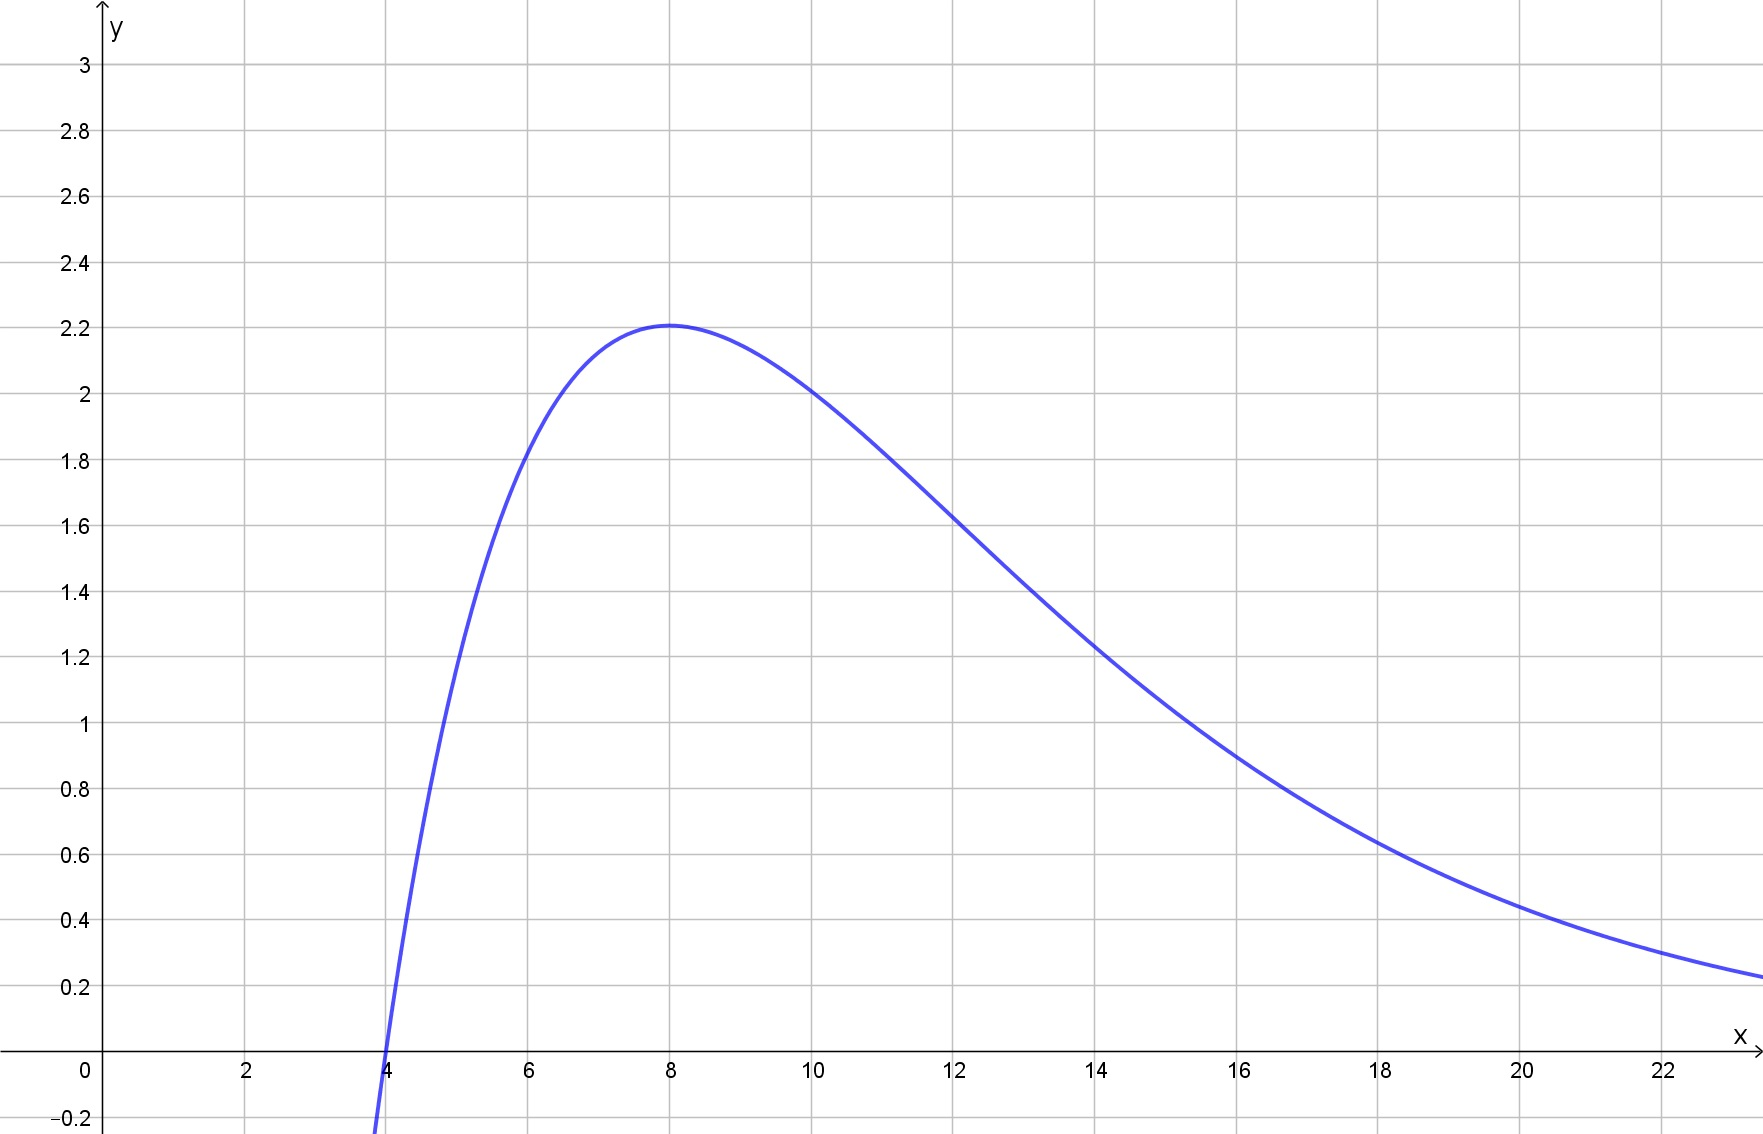
\includegraphics[width=0.7\textwidth]{../99_Bilder/01_ExpFkt/allgZsmhg.jpg}\\
			\end{center}
			\par\noindent
			(a) Bestimmen Sie \underline{anhand des Graphen der Ableitungsfunktion} die Extrem- und Wendestelle(n) der Funktion!\\
			(b) Zeigen Sie, dass es sich um eine Extremstelle vom Typ \textbf{TP} handelt und bestimmen Sie das relatives Minimum der Funktion.\\
			(c) Bestimmen Sie den y-Achsenabschnittswert und die Gleichung der Asymptote der Funktion und fertigen Sie eine Skizze des Graphen der Funktion an!\\
			(d) Interpretieren Sie den Verlauf des Graphen in Bezug auf die Situation!
		\end{framed}
		\begin{framed}
			\noindent
			\section*{Chemiewerk}
			Am 1. November ereignet sich im Chemiewerk Sandoz in Schweizerhalle ein Großbrand, bei dem große Mengen des Insektizids \grqq{}Disulfoton\grqq{} in den Rhein gelangt. Auch in Mainz konnten hohe Konzentrationen gemessen werden. Die Entwicklung der Konzentration über den Zeitverlauf in Mainz kann durch \[f(x) = e^{-0,2x}\cdot{}20\cdot{}x\] modelliert werden.\\
			(\(x\)x in Tagen nach dem Großbrand, \(f(x)\) in \(\mu{}g/Liter\))\\
			\par\noindent
			\rule{\textwidth}{0.1pt}\\
			Bestimmen Sie die Nullstellen, Extrem- und Wendestellen. Geben Sie zudem das Verhalten der Funktionswerte für x gegen Unendlich.\\
			Fertigen Sie anschließend eine Skizze des Graphen an, an dem Sie die Entwicklung der Konzentration erläutern!
		\end{framed}
		\begin{framed}
			\noindent
			\section*{Haushalt}
			Mit \(f(x) = (2x-40)\cdot{}e^{-0,2x+4}\) ist die Entwicklung des Finanzhaushalts einer Kleinstadt gegeben.\\
			\par\noindent
			(\(x\): in Jahren, \(0:= 1998\), \(y = \) in Mio. Euro)\\
			\par\noindent
			\rule{\textwidth}{0.1pt}\\
			Bestimmen Sie Nullstellen, Extrem- und Wendestellen und das Verhalten der Funktionswerte für x gegen Unendlich.\\
			Fertigen Sie anschließend eine Skizze des Graphen an, an dem Sie die Entwicklung des Haushalts ablesen können!
		\end{framed}
		\begin{framed}
			\noindent
			\section*{Antikörper}
			Einem Patienten mit einer schweren Virusinfektion werden Antikörper injiziert (\textit{passive Immunisierung}). Die \underline{Entwicklung des Antikörper-Bestands im Blut} lässt sich durch die mit \[f(x) = 20x\cdot{}e^{-0,5x}\] gegebenen Funktion angegeben.\\
			(\(x\): in Monaten; \(0:=\) Zeitpunkt der Injektion; \(f(x)\) Antikörperkonzentration im Blut in Nanogramm (ng)).\\
			\par\noindent
			\rule{\textwidth}{0.1pt}\\
			(a) Bestimmen Sie die charakteristischen Eigenschaften der Funktion (Null-, Extrem- und Wendestelle und Asymptote falls Vorhanden) mit Hilfe der Differentialrechnung und beschreiben Sie die Entwicklung auf Basis dieser Ergebnisse!\\
			Hierzu kann auch ein Graph skizziert werden!\\
			\par\noindent
			(b) Berechnen Sie den Wert der Ableitung an der Stelle \(x=4\) und interpretieren Sie diesen situationsbezogen!
		\end{framed}
		\begin{framed}
			\section*{Standardaufgaben}
			\subsection{I}
			Mit \(f(x) = e^{-4x} + 2x\) ist eine Funktion gegeben.\\
			Berechnen Sie den Hoch- bzw. Tiefpunkt, den y-Achsenabschnitt und die Asymptote.\\
			Fertigen Sie eine Skizze des Graphen an!
			\subsection{II}
			Eine Mensa einer großen Universität öffnet um 09:00 Uhr ihre Pforten. Die Zahl der Gäste, die sich in der Mensa befinden, lässt sich durch \[f(x) = (400x + 3600)\cdot{}e^{-0,5x}\] (\(x\) - Uhrzeit (z.B. \(x = 9\) entspricht 09:00 Uhr); \(y\) - Gäste in Tausend).\\
			\par\noindent
			\rule{\textwidth}{0.1pt}
			(a) Berechnen Sie die Extrem- und Wendestellen und interpretieren Sie die Stellen im Hinblick auf die Situation!\\
			\par\noindent
			(b) Fertigen Sie eine Skizze des Graphen an!
		\end{framed}
	\end{worksheet}
\end{document}